\section{Result interpretation and data}

\tab Here we will put all the results regarding hypertension and heart-disease from our dataset. We tested it with neural networks, with different algs and with lienarSCV and SCV ot see the diferences. \\
\tab The dataset percentage refeers to the amount of true test data in the dataset. If we let all the rows of the dataset, we will see that every classifier will predict false negative, and false positive, because there is few people with hypertension.\\
\tab We will manipulate the dataset in our favor, to be more precise in thesting the algorithms.\\


\tab Precision (also called positive predictive value) is the fraction of relevant instances among the retrieved instances, while recall (also known as sensitivity) is the fraction of relevant instances that have been retrieved over the total amount of relevant instances.Wiki.\\

\tab The F1 score is the harmonic average of the precision and recall, where an F1 score reaches its best value at 1 (perfect precision and recall) and worst at 0.\\

\tab ‘lbfgs’ is an optimizer in the family of quasi-Newton methods.\\
\tab ‘sgd’ refers to stochastic gradient descent.\\
\tab adam’ refers to a stochastic gradient-based optimizer proposed by Kingma, Diederik, and Jimmy Ba\\


\tab \tab \textbf{Confusion matrix}
\begin{center}
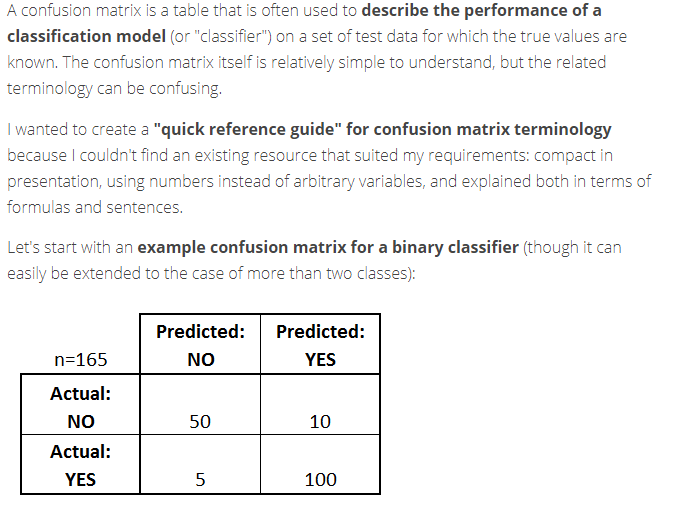
\includegraphics[scale=0.65]{confmatrix.png}
\end{center}

\begin{table}[h!]
\begin{center}
\caption{Results for predicting hypertension}
\label{tab:table1}
\begin{tabular}{c c c c c}
\textbf{Method and algorithm} & \textbf{Dataset percentage(true)} & \textbf{Precision }& \textbf{Recall }& \textbf{F1-score }\\
\hline
Neural Net - lbfgs & 45.6 & 0.69 & 0.69 & 0.69\\
Neural Net - lbfgs & 54.11 & 0.58 & 0.54 & 0.39\\
Neural Net - sgd & 45.6 & 0.53 & 0.52 & 0.38\\
Neural Net - sgd & 54.11 & 0.50 & 0.54 & 0.39\\
Neural Net - adam & 45.6 & 0.57 & 0.53 & 0.37 \\
Neural Net - adam & 54.11 & 0.58 & 0.50 & 0.42 \\
All data NN-adam & 0.09 & 0.82 & 0.89 & 0.83 \\
\end{tabular}
\end{center}
\end{table}

\begingroup\makeatletter\def\@currenvir{verbatim}
\verbatim
 Where confusion matrix of 1.\\
\[414, 157\],\\
\[183, 338\]\\

\tab confusion matrix of 2.\\
\[ 7, 395\],\\
\[ 4, 461\]\\

\tab confusion of 3.
\[558, 13\],\\
\[506, 15\]\\

\tab confusion of 4.
\[ 6, 396\],\\
\[ 7, 458\]\\

\tab conf of 5.
\[566, 5\],\\
\[513, 8\]\\

\tab conf of 6.
\[368, 34\]\\
\[397, 68\]\\
\end{verbatim}


\tab Here we see that there is a kind of good prediction , regarding the small sample of the dataset. Ofc, if we were to put all 50k rows in we will get 95 per cent prediction but only because the neural network have been trained to predict all values false because of dataset having few 5-10 per cent values of true in the test data.\\


\begin{table}[h!]
\begin{center}
\caption{Results for predicting heart-disease}
\label{tab:table2}
\begin{tabular}{c c c c c} 
\textbf{Method and algorithm} & \textbf{Dataset percentage(true)} & \textbf{Precision }& \textbf{Recall }& \textbf{F1-score }\\
\hline
Neural Net - lbfgs & 45.6 & 0.41 & 0.64 & 0.50 \\
Neural Net - lbfgs & 54.11 & 0.53 & 0.73 & 0.61 \\
Neural Net - sgd & 45.6 & 0.63 & 0.64 & 0.51\\
Neural Net - sgd & 54.11 & 0.62 & 0.73 & 0.61\\
Neural Net - adam & 45.6 & 0.66 & 0.44 & 0.37 \\
Neural Net - adam & 54.11 & 0.67 & 0.73 & 0.64 \\
All data NN-adam & 0.09 & 0.91 & 0.95 & 0.93 \\
\end{tabular}
\end{center}
\end{table}


\begingroup\makeatletter\def\@currenvir{verbatim}
\verbatim
Where confusion matrix of 1.\\
\[411, 0\],\\
\[233, 0\]\\

\tab confusion matrix of 2.\\
\[632, 0\],\\
\[237, 0\]\\

\tab confusion of 3.
\[409, 2\],\\
\[230, 3\]\\

\tab confusion of 4.
\[630, 2\],\\
\[236, 1\]\\

\tab conf of 5.
\[ 67, 344\],\\
\[ 16, 217\]\\

\tab conf of 6.
\[617, 15\],\\
\[223, 14\]\\

\tab conf of 7.
\[3554, 1\],\\
\[ 172, 0\]\\

\end{verbatim}



\section{Conclusions}

\tab The default solver ‘adam’ works pretty well on relatively large datasets (with thousands of training samples or more) in terms of both training time and validation score. For small datasets, however, ‘lbfgs’ can converge faster and perform better.Skit.\\

\tab Here we see that there is a kind of good prediction , regarding the small sample of the dataset. Ofc, if we were to put all 50k rows in we will get 95 per cent prediction but only because the neural network have been trained to predict all values false positive because of dataset having few 5-10 per cent values of true in the test data.\\

\tab One fact, if we add hidden layers of neurons, the values will start to converge rapidily to 80+ prediction and go into false positive values, like we said in the upper paragraph.\\